\documentclass{article}


% if you need to pass options to natbib, use, e.g.:
%     \PassOptionsToPackage{numbers, compress}{natbib}
% before loading neurips_2022


% ready for submission
\usepackage[final]{neurips_2022}


% to compile a preprint version, e.g., for submission to arXiv, add add the
% [preprint] option:
%     \usepackage[preprint]{neurips_2022}


% to compile a camera-ready version, add the [final] option, e.g.:
%     \usepackage[final]{neurips_2022}


% to avoid loading the natbib package, add option nonatbib:
%    \usepackage[nonatbib]{neurips_2022}


\usepackage[utf8]{inputenc} % allow utf-8 input
\usepackage[T1]{fontenc}    % use 8-bit T1 fonts
\usepackage{hyperref}       % hyperlinks
\usepackage{url}            % simple URL typesetting
\usepackage{booktabs}       % professional-quality tables
\usepackage{amsfonts}       % blackboard math symbols
\usepackage{nicefrac}       % compact symbols for 1/2, etc.
\usepackage{microtype}      % microtypography
\usepackage{xcolor}         % colors
\usepackage{graphicx}


\title{Managing the Whole Research Process on GitHub}


% The \author macro works with any number of authors. There are two commands
% used to separate the names and addresses of multiple authors: \And and \AND.
%
% Using \And between authors leaves it to LaTeX to determine where to break the
% lines. Using \AND forces a line break at that point. So, if LaTeX puts 3 of 4
% authors names on the first line, and the last on the second line, try using
% \AND instead of \And before the third author name.


\author{%
https://github.com/t46/github-research-management/graphs/contributors
\thanks{
  LaTeX source is available at 
  \href{https://github.com/t46/github-research-management}.
  }
}


\begin{document}


\maketitle


\begin{abstract}
  This is a position paper proposing the idea of managing the entire research process on GitHub. The current machine learning research community faces a variety of problems, such as poor quality and low reproducibility of peer review at international conferences. These problems are caused by a lack of transparency in the research process and a lack of accessibility, where not everyone can participate in any given process of research. Thus, we propose that any information that arises in the research process be posted on GitHub and that contributions to the research be managed like those in an open-source software project. This could provide a springboard for solving the challenges of machine learning through clarifying contributors, allowing fine-grained contributions, improving reproducibility, enabling post-publication peer review, enhancing diversity, and protecting ideas.
\end{abstract}


\section{Introduction}

\begin{figure}[htb]
    \centering
    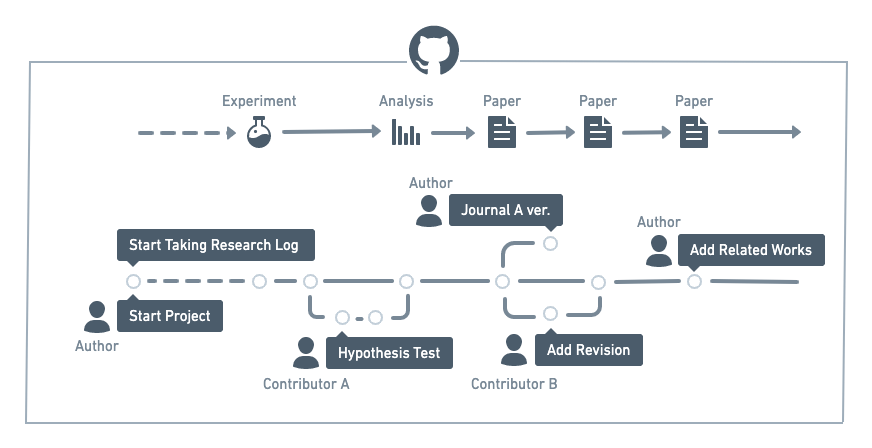
\includegraphics[width=\linewidth]{figs/GitHubResearchManagement.png}
    \caption{Conceptual diagram of managing research on GitHub. All intermediate outputs of the research process are placed on GitHub. Each contribution in the study is represented as a commit on GitHub, and authors can incorporate contributions from any contributor by accepting pull requests.}
    \label{fig:conceptual_diagram}
\end{figure}

The machine learning community faces several challenges, such as replication difficulty \cite{raff2019step} and the low quality of peer reviews \cite{cortes2021inconsistency}. Solving these challenges will ensure more reliable knowledge production and quality of knowledge. Also, making it easier for researchers to share knowledge and contribute to the others’ research can accelerate knowledge production. Enabling these is essential for optimized human knowledge production.

An idea to make these possible is to manage research in a public repository on GitHub, a Git repository hosting service \footnote{https://github.com/}. We know that experimental code is published on GitHub in machine learning research community. On the other hand, we propose to manage all intermediate outputs of the research process on GitHub, from the determination of the research topic to the post-publication paper. Literally, all intermediate products, including information about how researchers found the literature, what they thought, what initial experiments they did, etc. In addition, we propose that the progress of the research itself and the maintenance/management of the research results be done in a manner that mimics the way software open source projects proceed. 

Managing research on GitHub is a very simple proposal, but it would provide one prototype for solving many of the problems facing the machine learning research community. Specifically, managing research on GitHub would bring about the following benefits: clarifying contributors, allowing for contributions in a finer scale, improving reproducibility, enabling post-publication peer review (PPPR), embracing diversity, and protecting research ideas.

\section{Proposed Idea}
As mentioned in the previous section, we suggest that literally the entire research process be done on GitHub whenever possible. The first step is to create a research log. This can be in any format, e.g. markdown file. Then, since the stage of deciding on a research topic, you will publish it to the public repository on GitHub. Then, via \textit{commits} in GitHub, you record each process of the research in the research log, e.g., wherein the material you consulted and what ideas you got.

You also put on GitHub all intermediate outputs generated during the research. For example, the experimental conditions, the log files output for debugging, the results of numerical calculations, the results of pilot studies, and all other intermediate products.

When you start writing a paper (some people write it from the beginning of the research, others at the end), you also upload its latex file and all the files and data needed to compile it. Once the paper has passed peer review, you create a branch with the name of the journal/international conference. Then, in the main branch, you will continue to revise and update the paper. Issues that were not addressed in the peer review or that should be improved upon will be created as \textit{issues}. You will then continue to revise the paper by addressing these issues even after the paper is published. You accept contributions from anyone as \textit{pull requests}, both during the paper is written and after the paper is published.

\section{The Benefits of Managing Research on GitHub}

\subsection{GitHub clarifies contributors}
The first advantage is that managing research on GitHub clarifies who contributed and how. Currently, the most common way to express research contributions is to indicate the name of the author on the paper and to give implicit meaning to the order of the authors. However, this makes it difficult for a reader to know who contributed and how much; the contributions of the second and third authors may be far apart, or they may be almost the same. It may also specify what each author did but still does not show enough specific information to reproduce what was done in the research process. At best, they may say that they ``did the calculations'' or ``wrote the text''.

Suppose that all discussions and revisions of the manuscript are on GitHub. Then, the commit history can be traced to show who contributed to what part of the research process at a glance. Even if the authors’ names are not listed in the paper, the history on GitHub makes it clear to everyone the appropriate allocation of credit for the research.

This might, for example, eliminate gift-authorship problems \cite{grieger2005authorship}. Or it may solve the problem of how to order author names in a collaborative research project. It may also address the plagiarism issue \cite{anderson2011problem}. This is because these are the problems that one’s contribution is not recognized in the publication. 

\subsection{GitHub allows for finer contributions}
The second advantage is that on a more granular basis you can contribute to research and publish research results. Currently, those with smaller contributions are not included as authors in research papers. Even if they are included, it is common to mention them just in acknowledgments. However, if it were possible to contribute to research by commits on GitHub, these small contributions that have not been visualized so far would be visualized on the log of the research.

For example, someone good at statistical analysis may be able to commit only to the statistical analysis part. Or someone good at writing may contribute to the paper writing. Furthermore, minor typo corrections, short advice, and help for calculation are also visualized as contributions. 

Furthermore, enabling contribution on a per-commit basis means that citations will be available on a per-commit hash basis, not just on a per-article basis. This may lead to more direct recognition of individual contributions rather than papers. Citing a commit hash might make it possible to refer to specific ideas, results of experiments, problem formulation, etc. These would allow researchers to utilize multiple talents more effectively in their research.

\subsection{GitHub enables post-publication peer review}
The third advantage is that it may address the review crisis, which is a problem in machine learning research \cite{russo2021some}. To begin with, the number of scientific papers published is increasing rapidly \cite{bornmann2015growth}. In particular, because of the recent machine learning boom, there are not enough reviewers for the increasing number of researchers and papers in machine learning research. Because of an insufficient number of reviewers, non-experts often review \cite{russo2021some}. Especially in the case of international conferences on machine learning, it is more difficult to ensure the quality of peer review because of the limited review period. Also, because of the fast research cycle in machine learning, several important international conferences are held throughout the year \cite{deadlines}. Therefore, the peer review period for other conferences often overlaps with the preparation period for submitting your new paper to another conference, meaning that you have even less time to spend on peer review. These factors result in the decline and variation in the quality of reviews.

One possible solution to this problem of review quality is PPPR \cite{knoepfler2015reviewing}. PPPR is an attempt to ensure the validity of papers by evaluating the results after publication. The problem with the current machine learning peer review system is that papers are only evaluated by a specific person in a period of time. On the contrary, in a PPPR system, the quality of a paper is continuously evaluated by several peers for a long period of time after publication. This system seems to make sense, given that science is the activity of making certain that knowledge is irrefutable.

Managing the research on GitHub would help to achieve this PPPR. As we mentioned above, you place the LaTex file or markdown file of published paper on GitHub. Then, you accept corrections and comments on the file as pull requests. This will allow more people to participate in the evaluation of the published paper at any time and in any form they wish. This allows us to continually check the quality of research results on an ongoing basis.

Furthermore, this will lead to a return of the peer review process itself from "review to accept or not" to what it should be, "evaluation of the quality of the research results. Managing research on GitHub might be the beginning of a shift away from the competition for the top journal to a system that evaluates what is truly useful for the production of human knowledge.

\subsection{GitHub improves reproducibility}
The fourth advantage is that it may lead to better reproducibility of research. As mentioned above, machine learning researchers publish their code on GitHub. However, information during the research process, such as ``when it didn't work'' and ``what hyperparameters were important,'' is lost in some final repositories, decreasing reproducibility of the support for the main argument \cite{raff2019step}. Even slight change in the code sometimes makes your experiment fails. This means you should repeat the same process of searching for conditions the original proposer probably went through. In addition, many heuristics are not described or emphasized in the paper. 

We suspect this is due to the current pressure in the machine learning community to publish positive results to get into good international conferences. Publishing all intermediate thoughts and outputs of the research process would allow researchers to avoid making the same mistake twice. This helps another researcher to assess the work's soundness since all intermediate outputs are public.

In addition, the logging research process may contribute to reducing questionable research practices. For example, it might reduce the number of HarKing by making it possible to compare the time stamp when the hypothesis was determined with the time stamp when the experimental results were obtained. These attempts could lead to more reproducible and transparent research practices.

Furthermore, since the experimental design is publicly available, something corresponding to pre-registration could also be done on GitHub. Pre-registration is also considered an effective way to reduce QRP, so this is another way to help advance science.

\subsection{GitHub embraces diversity}
The fifth advantage is that more diverse people can participate in a research project. Open collaboration does not care who a person is, what institution they belong to, or what their background is. It does not matter what race, social class, or educational background they have. Research collaboration through GitHub would mitigate the diversity problem many research communities face \cite{west2019discriminating}.

One of the reasons diversity is an issue is researchers must belong to an organization, and selection must be made to determine the organization's membership. If research is conducted through a web-based platform such as GitHub, researchers can collaborate without any kind of affiliation. For these reasons, the generalization of research on GitHub would be effective in increasing the diversity of the research ecosystem.

\subsection{GitHub protects research ideas}
The sixth advantage is that more people may be able to publish unpublished content without fear of plagiarism \cite{anderson2011problem}. Currently, researchers generally do not publish their ideas until they are in a paper. This is because they fear that their ideas will be stolen and published first. However, withholding information increases the risk of multiple people duplicating and doing the same thing at the same time, and issues that could be solved immediately by others may not be solved and may not lead to results. Therefore, withholding information slows down the progress of science.

As mentioned above, a research log on GitHub shows who was thinking of what ideas and when. Therefore, even if a similar research idea appears later, you can track who states it first by checking the commit history. Hence, more people would be willing to share knowledge with others without fear of having their idea stolen by someone else. 

Recently, there has been a growing discussion about tying research contributions to the blockchain to guarantee uniqueness (e.g. DeSci \cite{hamburg2021call}). However, it will take time for this to be practical. Starting by visualizing research contributions on GitHub would be a good idea since it is an easy way to start.

\section{Discussion}
In this paper, we introduced the idea of managing research on GitHub. Then, we explained that doing research on GitHub can solve a variety of machine learning problems. 

To put this into practice, it would be good to start by putting published papers on GitHub and accepting PPPRs. This is because it may provide a prescription for the serious problem of lack of reviewers despite the psychologically and practically low barrier to entry compared to others.

In addition, the use of OSF (Open Science Framework) \cite{foster2017open} to disclose the research process is gradually becoming more prevalent in other research fields, such as psychology. And you can connect OSF with GitHub \cite{osfgithub}. So, it may be a good idea to start by making OSF pervasive in machine learning research, and then gradually shift to managing it on GitHub.

This could be effectively extended to other scientific domains, not just machine learning. The machine learning research community is a desirable environment to experiment with new research styles because experimental code is already available, most papers are open access, and research cycles are fast. By testing various research methods in machine learning research and exporting the good ones to other scientific fields, the development of science as a whole would be accelerated.

\bibliographystyle{unsrt}
\bibliography{ref}

\end{document}